%==============================================================================
%  ARES: A Stateful, Human-in-the-Loop Multi-Agent Architecture for
%        Grounded Autonomous Research Synthesis
%
%  Self-contained LaTeX source. Build with:
%      pdflatex ARES_paper.tex
%      pdflatex ARES_paper.tex      % second pass resolves refs & TikZ
%
%  Uses only widely-available packages (texlive-latex-recommended /
%  texlive-latex-extra / texlive-pictures). No bibtex pass required — the
%  bibliography is embedded below. A parallel references.bib is provided for
%  those who prefer a bibtex/biblatex workflow.
%==============================================================================
\documentclass[10pt,twocolumn]{article}

\usepackage[a4paper,margin=0.75in]{geometry}
\usepackage[T1]{fontenc}
\usepackage{lmodern}
\usepackage{microtype}
\usepackage{amsmath,amssymb}
\usepackage{graphicx}
\usepackage{booktabs}
\usepackage{array}
\usepackage{enumitem}
\usepackage{xcolor}
\usepackage{listings}
\usepackage{algorithm}
\usepackage{algpseudocode}
\usepackage{tikz}
\usetikzlibrary{arrows.meta,positioning,shapes.geometric,fit,backgrounds,calc}
\usepackage[hidelinks]{hyperref}
\usepackage{caption}
\captionsetup{font=small,labelfont=bf}

% --- Colours / listing style -------------------------------------------------
\definecolor{aresblue}{RGB}{40,55,120}
\definecolor{aresgrey}{RGB}{95,99,104}
\definecolor{codebg}{RGB}{247,248,250}
\definecolor{codekw}{RGB}{170,20,110}
\definecolor{codecm}{RGB}{95,120,95}
\lstset{
  basicstyle=\ttfamily\scriptsize,
  backgroundcolor=\color{codebg},
  keywordstyle=\color{codekw}\bfseries,
  commentstyle=\color{codecm}\itshape,
  stringstyle=\color{aresblue},
  breaklines=true,
  columns=fullflexible,
  frame=single,
  rulecolor=\color{aresgrey!40},
  showstringspaces=false,
  language=Python,
  aboveskip=6pt,belowskip=4pt,
}

\newcommand{\ares}{\textsc{Ares}}
\newcommand{\code}[1]{\texttt{\small #1}}

% --- Title -------------------------------------------------------------------
\title{\vspace{-1.2em}\textbf{\ares{}: A Stateful, Human-in-the-Loop Multi-Agent
Architecture for Grounded Autonomous Research Synthesis}}

\author{%
  \normalsize Udit Sharma\\[2pt]
  \small \texttt{teamforgeguild@gmail.com}\\[2pt]
  \small \textit{Independent Research}
}
\date{}

%==============================================================================
\begin{document}
\maketitle

\begin{abstract}
\noindent
Large Language Model (LLM) ``research assistants'' are typically implemented as
single-shot, linear pipelines: a query is expanded, a few documents are
retrieved, and one prompt produces a summary. Such pipelines are brittle
(a single tool failure loses the entire run), opaque (the user cannot steer the
line of inquiry), and prone to hallucination (generation is only loosely tied to
retrieved evidence). We present \ares{} (\emph{Autonomous Research \&
Multi-Agent Evaluation Engine}), a stateful, graph-orchestrated system that
reframes automated literature synthesis as the coordinated behaviour of a small
\emph{simulated research team}. \ares{} (i) generates diverse analyst personas
and exposes a human-in-the-loop checkpoint to steer them before any expensive
work begins; (ii) fans out an independent, retrieval-grounded expert
\emph{interview} per persona using a map--reduce execution pattern; and (iii)
synthesises the resulting cited memos into a structured report. The system is
built on LangGraph and is engineered for resilience: bounded exponential-backoff
retries, schema-validated structured outputs with graceful fallbacks, custom
channel reducers that tolerate concurrent state writes, and SQLite-backed
checkpointing that makes long-horizon runs pausable and resumable. We describe a
message \emph{re-roling} technique that enables robust multi-turn dialogue when
both interlocutors are instantiated from the same LLM --- a common failure mode
for small and locally-hosted models --- and a strict citation-grounding scheme
with stable inline numbering. We discuss the architecture, its design rationale,
qualitative behaviour, limitations, and an evaluation agenda.
\end{abstract}

\vspace{0.4em}
\noindent\textbf{Keywords:} multi-agent systems, LLM orchestration, retrieval
augmented generation, human-in-the-loop, LangGraph, agentic workflows, research
automation.

%------------------------------------------------------------------------------
\section{Introduction}
\label{sec:intro}

The rapid capability growth of instruction-tuned LLMs has made ``ask a question,
get a report'' tools ubiquitous. Yet the dominant implementation pattern remains
a \emph{single agent in a straight line}: expand the query, retrieve a handful of
passages, and emit one long generation. This pattern inherits three structural
weaknesses.

\begin{enumerate}[leftmargin=1.2em,itemsep=2pt]
  \item \textbf{Fragility.} A linear script has no notion of partial progress. If
  a search API rate-limits, a model call times out, or a structured-output parse
  fails, the whole run typically aborts and its intermediate work is discarded.
  \item \textbf{Opacity and lack of control.} The user provides a topic and
  receives an answer; there is no principled point at which they can inspect and
  redirect \emph{how} the topic will be investigated before compute is spent.
  \item \textbf{Weak grounding.} When retrieval and generation are only loosely
  coupled, the model freely interpolates unsupported claims, and citations --- if
  present --- often do not map to the passages actually used.
\end{enumerate}

\ares{} is a response to these weaknesses. Rather than a single agent, it
orchestrates a \emph{team}: a set of analyst personas, each of which interviews a
retrieval-grounded ``expert'' from a distinct angle, after which their findings
are reduced into a coherent report. The orchestration is expressed as an
explicit state graph, giving every intermediate artefact a durable home and every
control decision an inspectable edge.

\paragraph{Contributions.} This paper makes the following contributions.
\begin{enumerate}[leftmargin=1.2em,itemsep=2pt]
  \item \textbf{A phase-structured, graph-orchestrated architecture} that unifies
  (a) human-in-the-loop \emph{persona steering}, (b) a reusable interview
  sub-graph, and (c) a parallel map--reduce fan-out over personas within a single
  compiled, checkpointed graph (Section~\ref{sec:arch}).
  \item \textbf{A message re-roling technique} (\code{build\_dialogue}) that lets
  a single LLM sustain a coherent multi-turn interview \emph{with itself} by
  reconstructing a strict, role-alternating transcript per call --- addressing an
  empirical failure mode of small/local models (Section~\ref{sec:reroling}).
  \item \textbf{A resilience layer} combining bounded-retry invocation, structured
  outputs with typed fallbacks, and a concurrency-tolerant channel reducer that
  together enable fault-tolerant, resumable long-horizon runs over an
  SQLite checkpoint store (Section~\ref{sec:resilience}).
  \item \textbf{A strict retrieval-grounding and citation scheme} with stable
  inline numbering that constrains the expert to retrieved evidence and preserves
  a faithful source list into the final memo (Section~\ref{sec:grounding}).
\end{enumerate}

\ares{} is provider-agnostic (cloud NVIDIA NIM endpoints or fully-local Ollama),
retrieval-agnostic (Wikipedia plus DuckDuckGo or Tavily), and ships as a
single, containerised, dependency-light Python application.

%------------------------------------------------------------------------------
\section{Background and Related Work}
\label{sec:related}

\paragraph{Agentic LLM workflows.} A large body of recent work equips LLMs with
tools, memory, and iterative control loops. The ReAct paradigm interleaves
reasoning traces with tool actions~\cite{yao2023react}; reflection-style methods
add self-critique to improve robustness~\cite{shinn2023reflexion}. \ares{}
adopts the \emph{explicit-graph} view of agent control rather than a free-form
scratchpad: control flow is a compiled directed graph, which makes checkpointing,
interruption, and resumption first-class rather than emergent.

\paragraph{Multi-agent collaboration.} Frameworks such as generative-agent
societies~\cite{park2023generative} and role-playing conversational
frameworks~\cite{li2023camel,wu2023autogen} show that decomposing a task across
specialised roles can outperform a single monolithic agent. \ares{} follows this
intuition but constrains it: personas are not free-roaming chat participants but
\emph{interviewers} whose counterpart (the expert) is hard-limited to retrieved
context, trading open-ended emergence for grounding and reproducibility.

\paragraph{Retrieval-augmented generation (RAG).} RAG couples a parametric model
with a non-parametric retriever to reduce hallucination and inject fresh
knowledge~\cite{lewis2020rag}. \ares{} applies RAG \emph{per interview turn}: each
analyst question is rewritten into a search query, evidence is retrieved and
merged into a stably-numbered context window, and the expert is instructed to
answer using only that context with inline citations.

\paragraph{Human-in-the-loop (HITL) control.} Keeping a human in the decision
loop improves alignment and trust in automated systems. \ares{} places the human
at the highest-leverage point --- \emph{after} personas are proposed but
\emph{before} any interviews run --- so a small amount of human judgement steers a
large amount of downstream compute.

\paragraph{Graph orchestration substrate.} \ares{} is implemented on
LangGraph~\cite{langgraph}, which provides a \code{StateGraph} abstraction with
typed state channels, conditional edges, the \code{Send} primitive for dynamic
fan-out, compiled interruption points, and pluggable checkpointers. Our
contribution is not the substrate but the \emph{architecture} composed on top of
it and the engineering techniques that make it robust in practice.

%------------------------------------------------------------------------------
\section{System Architecture}
\label{sec:arch}

\ares{} is organised into four phases. Phases~1--3 are compiled into a single
master graph; Phase~4 is the interactive driver that streams the graph to a
terminal UI. Figure~\ref{fig:arch} shows the control flow.

\begin{figure*}[t]
\centering
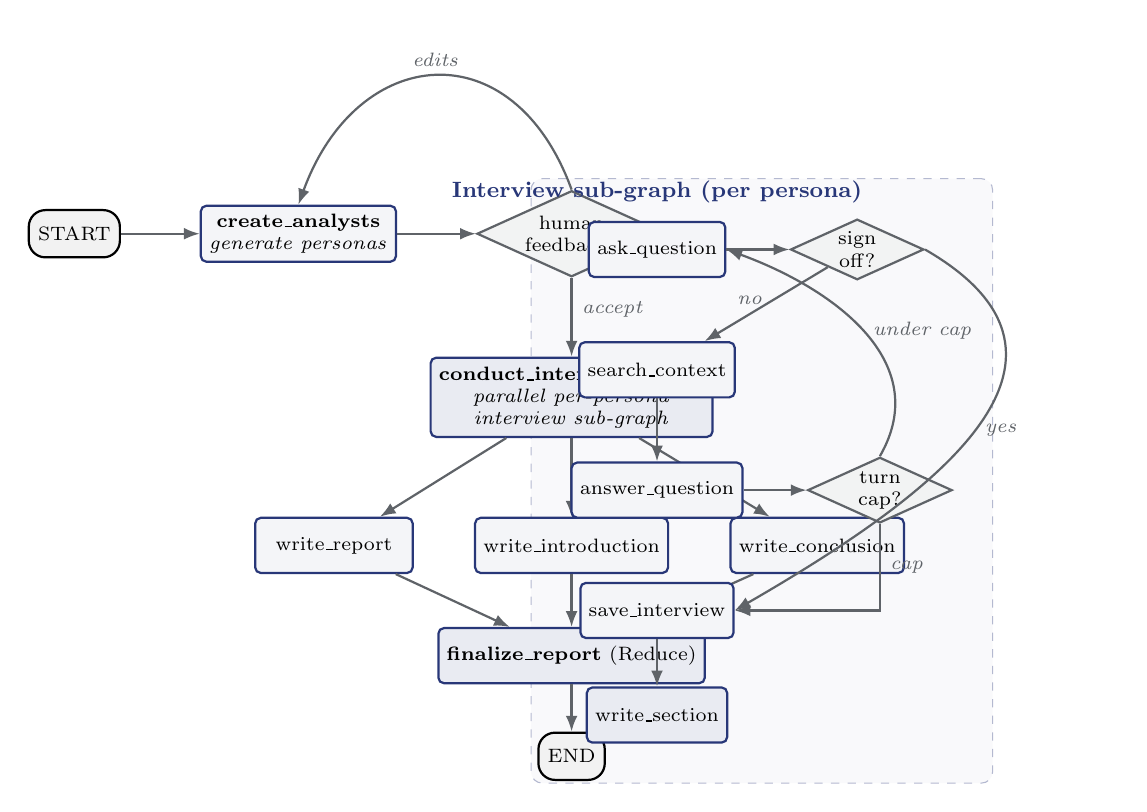
\begin{tikzpicture}[
  node distance=6mm and 10mm,
  every node/.style={font=\scriptsize},
  box/.style={draw=aresblue,thick,rounded corners=2pt,fill=aresblue!5,
              minimum height=7mm,minimum width=20mm,align=center,inner sep=3pt},
  dec/.style={draw=aresgrey,thick,diamond,aspect=2.2,fill=aresgrey!8,
              align=center,inner sep=1pt},
  term/.style={draw,thick,rounded corners=6pt,fill=black!5,minimum height=6mm},
  flow/.style={-{Latex[length=2mm]},thick,aresgrey},
]
  \node[term] (start) {START};
  \node[box,right=of start] (ca) {\textbf{create\_analysts}\\\textit{generate personas}};
  \node[dec,right=of ca] (hf) {human\\feedback?};
  \node[box,below=10mm of hf,fill=aresblue!10] (ci)
       {\textbf{conduct\_interview} (Map)\\\textit{parallel per-persona}\\\textit{interview sub-graph}};

  \node[box,below left=10mm and 2mm of ci] (wr) {write\_report};
  \node[box,below=10mm of ci] (wi) {write\_introduction};
  \node[box,below right=10mm and 2mm of ci] (wc) {write\_conclusion};
  \node[box,below=24mm of ci,fill=aresblue!10] (fr) {\textbf{finalize\_report} (Reduce)};
  \node[term,below=6mm of fr] (end) {END};

  \draw[flow] (start) -- (ca);
  \draw[flow] (ca) -- (hf);
  \draw[flow] (hf.north) to[out=110,in=70,looseness=1.6] node[above]{\itshape edits} (ca.north);
  \draw[flow] (hf) -- node[right,pos=0.4]{\itshape accept} (ci);
  \draw[flow] (ci) -- (wr);
  \draw[flow] (ci) -- (wi);
  \draw[flow] (ci) -- (wc);
  \draw[flow] (wr) -- (fr);
  \draw[flow] (wi) -- (fr);
  \draw[flow] (wc) -- (fr);
  \draw[flow] (fr) -- (end);

  % Interview sub-graph inset
  \begin{scope}[shift={(7.4,-0.2)}]
    \node[box,minimum width=16mm] (aq) {ask\_question};
    \node[dec,right=8mm of aq] (cof) {sign\\off?};
    \node[box,below=8mm of aq,minimum width=16mm] (sc) {search\_context};
    \node[box,below=8mm of sc,minimum width=16mm] (an) {answer\_question};
    \node[dec,right=8mm of an] (rm) {turn\\cap?};
    \node[box,below=8mm of an,minimum width=16mm] (si) {save\_interview};
    \node[box,below=6mm of si,minimum width=16mm,fill=aresblue!10] (ws) {write\_section};
    \node[above=1mm of aq,aresblue] {\footnotesize\textbf{Interview sub-graph (per persona)}};

    \draw[flow] (aq) -- (cof);
    \draw[flow] (cof) -- node[left,pos=0.45]{\itshape no} (sc);
    \draw[flow] (sc) -- (an);
    \draw[flow] (an) -- (rm);
    \draw[flow] (rm.north) to[out=60,in=-20,looseness=1.1] node[right,pos=0.5]{\itshape under cap} (aq.east);
    \draw[flow] (rm) |- node[pos=0.25,right]{\itshape cap} (si);
    \draw[flow] (cof.east) to[out=-30,in=30,looseness=1.4] node[right,pos=0.5]{\itshape yes} (si.east);
    \draw[flow] (si) -- (ws);
  \end{scope}
  \begin{scope}[on background layer]
    \node[draw=aresblue!35,dashed,rounded corners,fit=(aq)(cof)(sc)(an)(rm)(si)(ws),
          inner sep=5mm,fill=aresblue!3] {};
  \end{scope}
\end{tikzpicture}
\caption{\ares{} control flow. Left: the master graph --- persona generation, a
human-in-the-loop checkpoint, a map--reduce fan-out over personas, and report
finalisation. Right: the reusable interview sub-graph run once per persona,
which loops question$\rightarrow$retrieve$\rightarrow$answer until an early
sign-off or a turn cap, then writes a cited memo.}
\label{fig:arch}
\end{figure*}

\subsection{State model}
Data flows through three typed state objects, each a LangGraph channel schema:
\code{GenerateAnalystsState} (topic, budget, feedback, personas),
\code{InterviewState} (the message transcript, accumulated sources, the persona,
and the emitted memo), and the top-level \code{ResearchGraphState} (personas plus
the collected memos and the report parts). Channels declare \emph{reducers} that
define how concurrent or repeated writes combine; this is central to the
map--reduce step and is discussed in Section~\ref{sec:resilience}.

\subsection{Phase 1: Analyst persona generation with HITL steering}
\label{sec:phase1}
Given a topic and a budget $N$ of analysts, \ares{} prompts the LLM under a
\emph{structured-output} constraint to return exactly a list of $N$ personas,
each with a name, affiliation, role, and a description of its focus and motives.
Personas are the pipeline's most consequential artefact --- every downstream
interview inherits one --- so this call is allowed to fail loudly (no silent
fallback) after its retries are exhausted.

Immediately after generation, the compiled graph \emph{interrupts before} a
deliberately empty \code{human\_feedback} node. This pause surfaces the proposed
personas to the user, who may (i) press enter to accept and proceed, or (ii)
supply free-text editorial feedback. Feedback is recorded onto the interrupted
node's state and routes the graph back to \code{create\_analysts}, which
regenerates personas \emph{conditioned on} the feedback. Any number of refinement
rounds is supported. Crucially, the interrupt is a property of the compiled graph
(\code{interrupt\_before=["human\_feedback"]}), not of the driver loop, so the
same checkpoint semantics hold whether the run is interactive, scripted, or
resumed from disk.

\subsection{Phase 2: The interview sub-graph}
\label{sec:phase2}
Each persona conducts an independent interview with an ``expert'' instantiated
from the same LLM. The sub-graph (Figure~\ref{fig:arch}, right) has five nodes:

\begin{description}[leftmargin=1em,itemsep=1pt]
  \item[\code{ask\_question}] The analyst, in character, asks one specific
  question, building on the prior answer. A sign-off sentinel signals it is done.
  \item[\code{search\_context}] The latest analyst question is deterministically
  located and rewritten into a clean search query; evidence is retrieved from
  Wikipedia and (optionally) the web (Section~\ref{sec:grounding}).
  \item[\code{answer\_question}] The expert answers using \emph{only} the numbered
  retrieved context, citing sources inline. A two-stage safety net guarantees a
  non-empty answer even if the model initially returns nothing.
  \item[\code{save\_interview}] The transcript is serialised into a clearly
  role-labelled form for the section writer.
  \item[\code{write\_section}] The interview is synthesised into a focused,
  cited markdown memo with a guaranteed \emph{Sources} block.
\end{description}

Two conditional edges govern the loop. After a question,
\code{continue\_or\_finish} ends the interview early if the analyst has signed off
(and at least one answer already exists, preventing a wasted final answer to a
goodbye); otherwise it proceeds to retrieval. After an answer,
\code{route\_messages} ends the interview once the number of expert answers
reaches the turn cap, else loops back for another question. Turn counting is
robust: it counts \emph{tagged expert answers}, not raw message length.

\subsection{Phase 3: Map--reduce over personas}
\label{sec:phase3}
Once personas are accepted, \code{initiate\_all\_interviews} performs the
\textbf{Map} step by emitting one LangGraph \code{Send} per persona, each
launching a fresh instance of the Phase-2 sub-graph with its own seeded
transcript and turn budget. These instances execute concurrently and write their
memos into a shared, append-reduced \code{sections} channel. The \textbf{Reduce}
step then fans the collected memos into three parallel writers --- body,
introduction, and conclusion --- and a final join node stitches them, with the
topic as title, into the delivered markdown report. Expressing fan-out with
\code{Send} (rather than a static list of edges) means the parallel width is
determined \emph{at runtime} by the number of accepted personas.

\subsection{Phase 4: Execution and terminal UI}
The driver streams the master graph and renders progress with the \code{rich}
library: a banner, a persona table, live question/answer panels, search
indicators, and a final rendered-markdown report. Every UI helper degrades
gracefully to plain \code{print} if \code{rich} is unavailable, and the console
is forced to UTF-8 so emoji/Unicode never crash on legacy Windows code pages. The
driver exposes CLI flags (topic, persona count, turns, output path, thread id,
\code{--no-feedback}) that each fall back to an \code{ARES\_*} environment
variable, making the same entry point usable interactively and in headless
pipelines.

%------------------------------------------------------------------------------
\section{Message Re-roling for Single-Model Dialogue}
\label{sec:reroling}

A subtle but decisive engineering problem arises because the analyst and the
expert are the \emph{same} underlying LLM playing two roles. LangGraph's
\code{MessagesState} stores the whole interview in one \code{messages} list. To
keep speaker attribution unambiguous, \ares{} stores \emph{both} sides as
\code{AIMessage}s and tags expert turns with \code{name="expert"}; only the
initial seed is a \code{HumanMessage}.

This internal representation, however, is not what a chat model expects at
inference time. Chat models are trained on strictly alternating
Human/Assistant turns and, empirically, small and locally-hosted models often
emit \emph{empty} completions when handed a history that does not end on a human
turn or that contains consecutive same-role messages. \ares{} resolves this with
\code{build\_dialogue}, which reconstructs a fresh, per-call transcript from the
appropriate perspective without ever mutating stored state:

\begin{itemize}[leftmargin=1.2em,itemsep=1pt]
  \item \textbf{Expert perspective:} analyst questions become \code{Human} turns,
  the expert's own answers become \code{AI} turns, and the seed is dropped so the
  list \emph{ends on the question to be answered}.
  \item \textbf{Analyst perspective:} expert answers become \code{Human} turns,
  the analyst's own questions become \code{AI} turns, and the seed is retained as
  the opening human turn.
\end{itemize}

Finally, \code{merge\_message\_runs} collapses any accidental consecutive
same-role turns into a strictly alternating sequence. The net effect is that,
regardless of which role is being generated, the model always receives a clean
conversation that terminates on a human turn --- the configuration under which
instruction-tuned chat models are most reliable. This technique is what makes
\ares{} runnable on modest local models, not only large hosted endpoints.

%------------------------------------------------------------------------------
\section{Retrieval Grounding and Citation}
\label{sec:grounding}

\ares{} treats the expert as a \emph{closed-book-turned-open-book} agent: it may
only use what retrieval provides. Three mechanisms enforce and preserve this.

\paragraph{Deterministic query construction.} Because the transcript is
all-\code{AIMessage}, asking the model to ``search the last question'' is
ambiguous. \ares{} instead walks the message list in reverse to
\emph{deterministically} select the latest untagged (analyst) message, then
rewrites it into a short query under a structured-output schema, with the raw
question text as a fallback.

\paragraph{Stable numbered context.} Retrieved passages (Wikipedia documents plus
optional web snippets) are de-duplicated by URL preserving first-seen order,
capped to a maximum count, and truncated to a per-source character budget. They
are then rendered as \code{[1] Source: \dots} blocks. The same numbering is used
both in the context handed to the expert and in the \emph{Sources} listing
emitted with the memo, so an inline \code{[2]} in the answer maps to a real,
listed source. Deferring the cap-and-number step to render time (while retaining
the full source list in state) keeps prompts within context limits without losing
provenance.

\paragraph{Instructional and structural guarantees.} The expert prompt forbids
external facts and requires inline \code{[n]} citations; the section writer is
constrained to synthesise from the transcript rather than invent facts; and if
the writer omits a \emph{Sources} block, \ares{} appends the numbered listing
programmatically. Grounding is thus enforced at the prompt level and
\emph{backstopped} at the code level.

%------------------------------------------------------------------------------
\section{Resilience, Concurrency, and Persistence}
\label{sec:resilience}

Long-horizon, multi-call agentic runs fail in many small ways. \ares{} is built
to survive them.

\paragraph{Bounded-retry invocation.} All model calls route through two wrappers.
\code{safe\_invoke} retries plain generations with exponential backoff and
re-raises only after exhausting attempts. \code{structured\_invoke} does the same
for schema-constrained calls but additionally accepts a \emph{typed fallback}:
non-critical structured calls (e.g. query rewriting) degrade to a safe default
instead of aborting the run, whereas critical calls (persona generation) omit the
fallback and are allowed to fail loudly. A transient-error classifier gives users
an actionable message (``is Ollama running?'', ``check your API key'') when the
backend is unreachable.

\paragraph{Concurrency-tolerant reducers.} The map step runs $N$ interview
sub-graphs in one super-step. Each echoes the same scalar \code{max\_num\_turns}
back to the parent, and a naive last-value channel rejects $N$ simultaneous
writes with an \code{InvalidUpdateError}. \ares{} defines a custom reducer,
\code{\_keep\_last}, that folds concurrent identical writes into a single value.
Accumulating channels (\code{sources}, \code{sections}) use additive reducers so
that parallel contributions \emph{merge} rather than clobber. Algorithm~\ref{alg:mapreduce}
sketches the pattern.

\paragraph{Checkpointing and resumption.} The master graph is compiled with an
SQLite checkpointer keyed by a \code{thread\_id}. Every super-step persists state
to disk, so a run can be interrupted --- by the HITL pause, a crash, or the user
--- and later \emph{resumed} by supplying the same thread id. If the SQLite extra
is unavailable, \ares{} falls back to an in-memory saver, preserving semantics for
a single process. A fresh random thread id per run prevents accidentally resuming
a completed run from the persistent store.

\begin{algorithm}[t]
\caption{Map--reduce over analyst personas}
\label{alg:mapreduce}
\begin{algorithmic}[1]
\Require topic $t$, personas $A=\{a_1,\dots,a_N\}$, turn cap $\tau$
\Statex \textbf{-- Map (parallel) --}
\ForAll{$a_i \in A$ \textbf{concurrently}}
  \State seed transcript with ``Start the interview: $t$''
  \State $m_i \gets \textproc{InterviewSubgraph}(a_i,\tau)$
       \Comment{cited memo}
  \State append $m_i$ to \code{sections} \Comment{additive reducer}
\EndFor
\Statex \textbf{-- Reduce (parallel writers, then join) --}
\State $B \gets \textproc{WriteBody}(\code{sections})$
\State $I \gets \textproc{WriteIntro}(t)$
\State $C \gets \textproc{WriteConclusion}(t)$
\State \Return $\textproc{Stitch}(t, I, B, C)$
\end{algorithmic}
\end{algorithm}

\paragraph{Provider and retrieval abstraction.} Only the active LLM provider's
package is imported and only its credential is validated, so a local Ollama run
never requires a cloud key and vice-versa. Web search is likewise pluggable
(DuckDuckGo by default and keyless, Tavily optionally, or disabled), and each
backend degrades to an empty result set rather than raising, so retrieval hiccups
never abort a run.

%------------------------------------------------------------------------------
\section{Implementation}
\label{sec:impl}

\ares{} is a single, self-documenting Python module ($\approx$1.1k lines)
depending on LangGraph, LangChain community loaders, a provider SDK, and
\code{rich}. Listing~\ref{lst:reduce} shows the concurrency-tolerant channel
declarations that make the map step correct. Table~\ref{tab:config} summarises
the runtime configuration surface. The project ships with a slim, non-root
Docker image and a Compose stack that can optionally run a fully-local Ollama
sidecar, so a reviewer can reproduce a run with a single command and no local
Python setup.

\begin{lstlisting}[caption={Typed state channels with reducers that make parallel
writes well-defined.},label={lst:reduce}]
class ResearchGraphState(TypedDict):
    topic: str
    max_analysts: int
    # fold N identical concurrent writes -> 1
    max_num_turns: Annotated[int, _keep_last]
    human_analyst_feedback: str
    analysts: List[Analyst]
    # parallel memos MERGE, not clobber
    sections: Annotated[list, operator.add]
    introduction: str
    content: str
    conclusion: str
    final_report: str
\end{lstlisting}

\begin{table}[t]
\centering
\caption{Selected runtime configuration (environment variables).}
\label{tab:config}
\small
\begin{tabular}{@{}p{0.30\columnwidth}p{0.60\columnwidth}@{}}
\toprule
\textbf{Variable} & \textbf{Role (default)} \\
\midrule
\code{LLM\_PROVIDER} & \code{nvidia} \textbar{} \code{ollama} (nvidia) \\
\code{NVIDIA\_MODEL} & NIM model id (llama-3.3-70b) \\
\code{OLLAMA\_MODEL} & local model (llama3.1:8b) \\
\code{CHECKPOINT\_BACKEND} & \code{sqlite} \textbar{} \code{memory} (sqlite) \\
\code{SEARCH\_BACKEND} & \code{duckduckgo}\,\textbar\,\code{tavily}\,\textbar\,\code{none} \\
\code{WEB\_MAX\_RESULTS} & web results/query (3) \\
\code{MAX\_SOURCES\_FOR\_EXPERT} & sources shown to expert (5) \\
\code{MAX\_SOURCE\_CHARS} & per-source char cap (1500) \\
\bottomrule
\end{tabular}
\end{table}

%------------------------------------------------------------------------------
\section{Qualitative Behaviour and Evaluation Agenda}
\label{sec:eval}

\ares{} is a systems contribution; a full quantitative study is future work.
Here we characterise its behaviour and lay out an evaluation protocol.

\paragraph{Observed behaviour.} On representative topics (e.g. renewable-energy
microgrids), \ares{} reliably (i) produces personas spanning complementary angles
(technical, financial, regulatory); (ii) drives multi-turn interviews in which
each expert answer carries inline citations that resolve to the listed sources;
and (iii) synthesises a structured report whose claims trace back to retrieved
evidence. The HITL step demonstrably changes the run: feedback such as ``add an
economist'' regenerates the persona set before any interview cost is incurred.

\paragraph{Proposed metrics.} We propose evaluating \ares{} along four axes:
\begin{enumerate}[leftmargin=1.2em,itemsep=1pt]
  \item \textbf{Citation faithfulness} --- the fraction of inline \code{[n]}
  citations whose associated claim is supported by source $n$ (human or
  LLM-as-judge adjudicated).
  \item \textbf{Coverage / diversity} --- semantic spread of persona foci and of
  the questions asked, versus a single-agent baseline.
  \item \textbf{Robustness} --- completion rate under injected faults (search
  timeouts, empty generations, parse failures) with and without the resilience
  layer.
  \item \textbf{Steerability} --- the effect of HITL feedback on final-report
  relevance, via A/B runs with and without the checkpoint.
\end{enumerate}

\paragraph{Baselines.} Natural comparators are (a) a single-shot RAG summariser,
(b) \ares{} with one persona and one turn (ablating the team), and (c) \ares{}
with the resilience layer disabled (ablating fault tolerance).

%------------------------------------------------------------------------------
\section{Limitations}
\label{sec:limits}

\ares{} inherits the limits of its components. Retrieval quality bounds answer
quality: a keyless web backend and short per-source budgets can miss or truncate
relevant evidence. The expert and analyst share one model, so systematic model
biases are correlated across roles rather than independent. Grounding is enforced
by instruction and structure but not \emph{proven}: a determined model can still
paraphrase beyond its sources, which is precisely why citation-faithfulness
measurement is prioritised as future work. Parallel fan-out multiplies token and
latency cost roughly linearly in the number of personas. Finally, the current
synthesis stage writes intro/body/conclusion independently; it does not yet
perform a global consistency or contradiction-resolution pass across memos.

%------------------------------------------------------------------------------
\section{Future Work}
\label{sec:future}

Priorities are: (i) the quantitative evaluation of Section~\ref{sec:eval},
including an automated citation-faithfulness harness; (ii) a cross-memo
reconciliation node that detects and resolves contradictions before finalisation;
(iii) heterogeneous role models (a stronger model for synthesis, a cheaper one
for interviews); (iv) richer retrieval (vector stores, PDF and arXiv ingestion,
recency-aware ranking); and (v) an evaluation/critique agent --- the ``E'' in
\ares{}'s name --- that scores each memo and can trigger targeted re-interviews,
closing an outer quality-control loop around the current pipeline.

%------------------------------------------------------------------------------
\section{Conclusion}
\label{sec:conclusion}

\ares{} reframes automated research synthesis from a fragile linear script into
the coordinated behaviour of a small, steerable, resilient research team. By
expressing the workflow as an explicit, checkpointed state graph, it earns
durable intermediate state, first-class interruption and resumption, and a
principled human-in-the-loop steering point. Its engineering contributions --- a
single-model dialogue re-roling technique, concurrency-tolerant channel reducers,
a retry-and-fallback resilience layer, and a strict numbered-citation grounding
scheme --- are individually small but collectively transform a demo-grade agent
into a system that survives real-world failures and remains transparent to its
user. We believe this ``simulated team on an explicit graph'' pattern is a
productive template for a broad class of long-horizon, evidence-grounded
LLM applications.

%------------------------------------------------------------------------------
\begin{thebibliography}{9}
\small
\bibitem{yao2023react}
S.~Yao \emph{et al.},
``ReAct: Synergizing Reasoning and Acting in Language Models,''
\emph{ICLR}, 2023.

\bibitem{shinn2023reflexion}
N.~Shinn \emph{et al.},
``Reflexion: Language Agents with Verbal Reinforcement Learning,''
\emph{NeurIPS}, 2023.

\bibitem{park2023generative}
J.~S.~Park \emph{et al.},
``Generative Agents: Interactive Simulacra of Human Behavior,''
\emph{UIST}, 2023.

\bibitem{li2023camel}
G.~Li \emph{et al.},
``CAMEL: Communicative Agents for `Mind' Exploration of Large Language Model
Society,'' \emph{NeurIPS}, 2023.

\bibitem{wu2023autogen}
Q.~Wu \emph{et al.},
``AutoGen: Enabling Next-Gen LLM Applications via Multi-Agent Conversation,''
\emph{arXiv:2308.08155}, 2023.

\bibitem{lewis2020rag}
P.~Lewis \emph{et al.},
``Retrieval-Augmented Generation for Knowledge-Intensive NLP Tasks,''
\emph{NeurIPS}, 2020.

\bibitem{langgraph}
LangChain, ``LangGraph: Building Stateful, Multi-Actor Applications with LLMs,''
\url{https://github.com/langchain-ai/langgraph}, 2024.

\bibitem{lewis2021kilt}
P.~Lewis \emph{et al.},
``KILT: a Benchmark for Knowledge Intensive Language Tasks,''
\emph{NAACL}, 2021.

\bibitem{es2023ragas}
S.~Es \emph{et al.},
``RAGAS: Automated Evaluation of Retrieval Augmented Generation,''
\emph{arXiv:2309.15217}, 2023.
\end{thebibliography}

\end{document}
